\subsubsection {}
\label{sec:analysis:research:backArch:monolith}

Монолитная архитектура предполагает развёртывание программног средства одним файлом (например, WAR фаил) или~архивом файлов (например, программа на~Rails), все модули ПС разрабатываются, развёртываются и~тестируются одновременно. Обычно при~реализации данного подхода, весь код программног средства использует одну базу данных. На~рисунке \ref{sec:analysis:research:arch:back:monolith} представлен пример организации монолитного ПС\cite{microservices:ma}.

\begin{figure}[h]
  \centering
    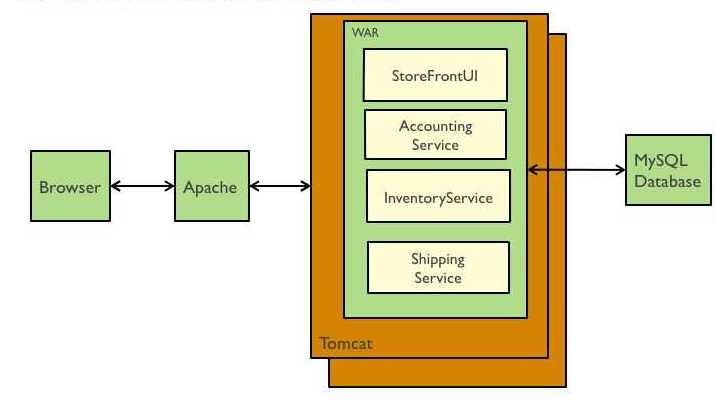
\includegraphics[width=1\textwidth]{inc/img/backend-monolith.jpg}
  \caption{Пример организации монолитного серверного ПС}
  \label{sec:analysis:research:arch:back:monolith}
\end{figure}

К плюсам подхода можно отнести:

\begin{enumerate}
	\item \emph{Простота в~разработке} -- целью современных \gls{ide} является поддержка монолитных приложений.
	\item \emph{Простота в~развёртывании} -- для~старта работы всего программног средства нужно лишь запустить один процесс с~подготовленным окружением.
	\item \emph{Простота в~масштабируемости} -- ПС масштабируется путём запуска дополнительных процессов, организованных при~помощи балансировщика нагрузки.
\end{enumerate}

Данный подход удобен до~определённого размера программного средства, однако, чем больше и~сложнее становится программное средство, тем существенней становятся следующие проблемы:

\begin{enumerate}
	\item \emph{Сложность поддержки} -- с~увеличением кодовой базы, увеличивается сложность ввода нового специалиста в~проект. Результатом является общее замедление разработки и~отсутствие возможности быстро ускорить разработку при~помощи привлечения дополнительных специалистов.
	\item \emph{Перегруженная \gls{ide}} -- хотя современные \gls{ide} и~ориентируеются на~монолитные ПС, большая кодовая база способна сильно замедлить работу \gls{ide}.
	\item Долгий запуск контейнера программного средства.
	\item \emph{Сложности при~масштабировании} -- на~определённом этапе, в~коде появляются слабые точки производительности. Часто таких точек несколько и~они трeбуют разные виды ресурсов (база, процессор, память), однако единственный способ масштабировать программное средство -- запускать новый процесс со всем ПС внутри, что~не позволяет точечно устранять проблемы.
	\item \emph{Привязанность к~технологическому стеку} -- монолитное ПС крайне сложно постепенно переводить на~новый технологический стек, а~единовременное полное портирование ПС -- опасный процесс, производящий огромное количество ошибок.
\end{enumerate}